\section{Experimental design}
\label{sec:experiment}

\subsection{Data and contamination}

The images come from STL-10~\cite{coates2011stl10}. Airplane, monkey, and truck
are the target classes. Each assigned label contains 100 images, and all
conditions within one repetition use the same target-class pools. Contamination
replaces clean images rather than increasing class size. The tested rates are
10\%, 20\%, and 30\%.

In the \emph{mixed} condition, contaminants are divided as evenly as possible
between the other two target classes. In the \emph{systematic} condition, the
error direction is fixed: monkey images receive the airplane label, truck
images receive the monkey label, and airplane images receive the truck label.
The \emph{unseen} condition inserts dog, car, and ship images into each target
label, balanced as closely as the selected rate allows.

\subsection{Training and evaluation}

Models were created and exported to Keras through Google Teachable
Machine~\cite{teachablemachine}. Every condition used 50 epochs, batch size 16,
and learning rate 0.001. The 538,608-parameter network accepts
$224\times224$ RGB input. Each condition was trained ten times, producing 100
model files. Repetitions 1--3 used one fixed set of training images.
Repetitions 4--10 used newly sampled 100-image target pools per class. Within
each repetition, the ten conditions shared those target pools. Teachable
Machine did not expose a training seed.

\begin{figure*}[t]
  \centering
  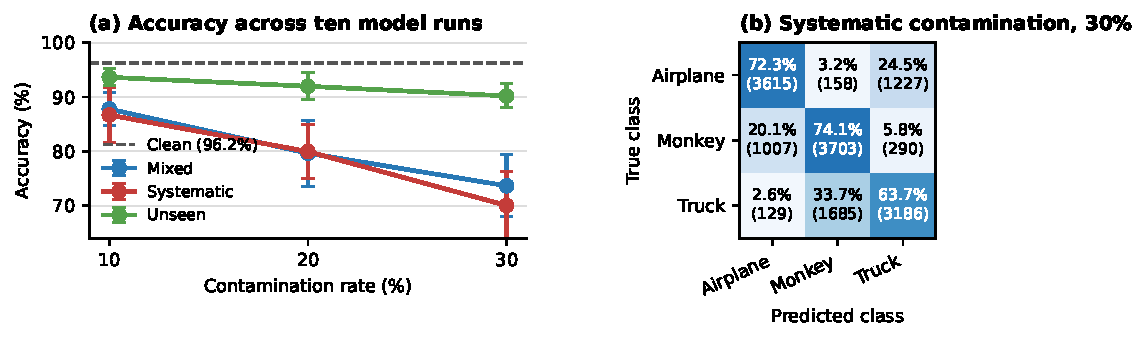
\includegraphics[width=0.96\textwidth]{figures/results_overview.pdf}
  \caption{\textbf{Left:} Mean test accuracy; bars show one sample standard
  deviation across ten trained models. \textbf{Right:} Aggregate row-normalized
  confusion matrix for 30\% systematic contamination. Counts combine all ten
  models and 5,000 predictions per true class.}
  \label{fig:results}
\end{figure*}

Each repetition used ten mutually disjoint STL-10 test sets with 50 clean
images per class. Repetitions 1--3 shared the original test suite;
repetitions 4--10 used repeat-specific suites. No test image was used for
training. Overlap across different repeat-specific suites was allowed. Images
were resized to $224\times224$ and normalized to $[-1,1]$. The analysis contains
1,000 model--test-set evaluations and 150,000 predictions. Scores were averaged
over ten sets; the reported mean and sample standard deviation were calculated
from the ten model means. Selection seeds were
20261114 (original) and 20261115 (extended). Evaluation used Python 3.10 with
TensorFlow 2.15, NumPy 1.26.4, and OpenCV 4.11.
